\documentclass[12pt, a4paper, oneside, romanian]{teza-upb}
\setcounter{secnumdepth}{3}
\setcounter{tocdepth}{3}
\usepackage[romanian]{babel}
\usepackage{graphicx}
\usepackage{float}
\usepackage[
  bookmarksnumbered,
  bookmarks,
  bookmarksopen=true,
  pdftitle={Dizertatie},
  linktocpage]{hyperref}
\singlespacing
\begin{document}
\author{Andrei Mihăescu}

\title{Arhitecturi software orientate pe servicii}


\facultatea{Facultatea de Electronică, Telecomunicații și Tehnologia Informației}
\tiplucrare{cercetare}
\domeniu{Electronică, Telecomunicații și Tehnologia Informației}
\catedra{Telecomunicații}
\campus{Leu} 
\program{Tehnologii Software Avansate pentru Comunicatii}
\titlulobtinut{Master}
\director{Conf. Dr. Eduard Popivici} 

\submissionmonth{Iunie} 
\submissionyear{2016} 

\beforepreface
\listoffigures
\listoftables
\abbreviations{ 
BDFU - Big Design Upfront \\
COBRA - Common Object Request Broker Architecture \\
COM - Common Object Model \\
DCOM - Distributed Common Object Model  \\
DDD - Domain-Driven Design \\
DRY - Don't repeat yourself \\
EJB - Enterprise Java Beans \\ 
ESB - Enterprise Service Bus \\
ISB - Internet Service Bus \\ 
JIT - Just in time \\
LOB - Line-of-business \\
MVC - Model View Controller \\
P2P - Peer-to-Peer \\
QA - Quality Assurance \\ 
RPC - Remote Procedure Call \\
SOA - Service Oriented Architecture \\
UML - Unified Modelling Language \\
URI - Uniform Resource Identifiers \\
YAGNI - You ain't gonna need it \\


}

%\preface{}
\afterpreface 

\chapter{Introducere}
\section{Ce este o arhitectura software?}
Arhitectura software reprezintă procesul de definire a unei soluții structurate care îndeplinește toate cerințele tehnice și operaționale, totodata optimizând metrici comune de calitate precum performanța, securitatea si facila gestiune. Aceasta presupune o serie de decizii bazate pe o gamă largă de factori fiecare din aceștia având un impact considerabil asupra calității, performanței, gestionabilitații și bunei funcționarii a aplicației.

Philippe Kruchten, Grady Booch, Kurt Bittner și Rich Reitman au derivat și rafinat definiția arhitecturii software bazându-se pe munca lui Mark Shaw si David Garlan (Shawn and Garlan 1996). Definiția lor este următoarea:

"Arhitectura software înglobează setul deciziilor semnificative legate de organizarea unui sistem software ce includ selectarea elementelor structurale și a interfețelor din care sistemul este compus; comportamentul așa cum reiese din interacțiunea acestor elemente; compunerea acestor elemente structurale și comportamentale în subsisteme mai mari; și un stil arhitectural care guvernează această organizare. Arhitectura software implică constrângeri și compromisuri legate de funcționalitate, utilitate, robustețe, performanță, reutilizare, inteligibilitate, economie, tehnice și estetice."

În cartea \emph{"Patterns of Enterprise Application Architecture"}, Martin Fowler evidențiază câteva teme recurente explicând conceptul de arhitectură. El identifică aceste teme dupa cum urmează: "Descompunerea de nivel înalt a unui sistem în parți componente; deciziile care sunt dificil de schimbat; există multe arhitecturi intr-un sistem; ceea ce este arhitectural important se poate schimba de-a lungul ciclului de viata al sistemului; și, la final, arhitectura se rezumă la lucrurile importante."

În cartea \emph{"Software Architecture in Practice (2nd edition)"} Bass, Clements, and Kazman definesc arhitectura astfel: "Arhitectura software a unui program sau a unui sistem de calcul reprezintă structura sau structurile, ce înglobează elementele software, proprietățile lor vizibile către exterior și relația între acestea. Arhitectura se preocupă cu partea public a interfețelor; detaliile private ale elementelor - cele ce sunt strict legate de implementarea internă - nu sunt legate de arhitectură."

\newpage
\section{De ce este arhitectura importantă ?}
Ca orice structură complexă, software-ul trebuie construit pe o bază solidă. Neluarea în considerare a anumitor scenarii cheie, cât și ignorarea anumitor probleme comune de design pot pune aplicația în pericol. Uneltele și platformele moderne ajută la construirea aplicațiilor, însă nu pot înlocui nevoia unuei proiectării atente a aplicației, bazată pe scenarii și cerințe. Riscurile pe care le presupune o arhitectură slab gândită sunt instabilitatea, inabilitatea de a susține cerințele actuale și viitoare de business sau dificultatea de instalare și gestiune într-un mediu de producție.

Un sistem ar trebui proiectat luând în considerare utilizatorul, infrastructura și obiectivele de business. Pentru fiecare din aceste arii, trebuie gândite scenarii cheie, identificate proprietațile relevante și arii cheie de satisfacție și desatisfacție. Unde este posibil, este indicat sa se stabilească metrici precise care vor putea fii evaluate pentru a măsura succesul fiecărei arii.

Cel mai probabil vor exista compromisuri și un echilibru trebuie găsit între cerințele concurente din aceste trei arii. De exemplu experiența utilizatorului, este adesea o funcție de business și infrastructură și schimbările într-una din zone o poate drastic afecta. În mod similar, schimbările la nivelul experienței de utilizare pot avea impact la nivelul infrastructurii și business. Performanța ar putea fi importantă din punct de vedere business și al utilizatorului, dar administratorul de sistem poate nu avea mijloacele financiare pentru a atinge obiectivele în 100\% din timp. Un compromis ar fi să atingă obiectivele 80\% din timp.

Rolul arhitecturii este acela de a defini modul în care elemente majore și componente din cadrul aplicației sunt folosite sau interacționează între ele. Selectarea structurilor de date și a algoritmilor, cât și detaliile de implementare specifice fiecărei componente nu sunt de interes pentru proiectare. Problemele de arhitectură și proiectare de multe ori se intercalează. In unele cazuri, deciziile țin mai mult de arhitectură. In altele, în schimb țin mai mult de proiectare și de cum acestea contribuie la realizarea arhitecturii.

\section{Obiectivele arhitecturii software}

Arhitectura software urmărește să găsească un compromis între specificațiile de business și cele tehnice înțelegând cazurile de utilizare și apoi găsind căi de implementare. Obiectivele arhitecturii sunt acelea de a găsi cerințele care influențează structura aplicației. O arhitectură bine realizată reduce riscurile de business asociate cu construirea unei soluții tehnice. Un design bun este suficient de flexibil ca să poate gestiona devierile de la tehnologiile software si hardwre care pot apărea în timp, cât și cerințele utilizatorilor. Un arhitect trebuie să ia in considerare efectul global al deciziilor de proiectare, cât și compromisurile inerente între factorii de perfomanță, dar și cele cu privire la utilizator, infrastructură și cerințele de business.

\newpage
\section{Principii arhitecturale cheie}
Pentru proiectarea unei arhitecturii următoarele principii cheie ar trebui luate în calcul:
\begin{itemize}
	\item \textbf{Arhitectura trebuie sa fie concepută pentru a suporta schimbări, nu pentru a rămâne neschimbătă.} Întotdeauna trebuie luat în calcul cum aplicația s-ar putea modifica de-a lungul timpului pentru a putea răspunde noilor cerințe și provocări.
	\item \textbf{Modelarea trebuie facută pentru reduce riscul.} Este indicată folosirea uneltelor de proiectare, a sistemelor de modelare precum \textbf{UML -} \emph{Unified Modelling Language} și a vizualizare unde este cazul pentru a putea evidenția cerințele și a deciziile arhitecturale și de proiectare, analizându-le impactul.
	\item \textbf{Folosirea modelelor și a uneltelor de vizualizare pentru comunicare si colaborare.} Comunicarea eficientă a designului, a deciziilor luate și schimbărilor necesare este necesară unei arhitecturi bune. Este recomandată folosirea modelelor, a vederilor și a altor mijloace de vizualire a arhitecturii pentru a comunica și impărtăși eficient ideile cu clienții, rezultând astfel într-o comunicare rapidă a schimbărilor de proiectare.
	\item \textbf{Identificarea deciziilor tehnice cheie.} Este esențiala înțelegerea deciziilor tehnice cheie pentru evitarea greșelilor comune. Investirea în luarea acestor decizii bine de prima dată este importantă pentru a obține un design flexibil și foarte puțin expus riscului de a fi afectat de viitoare schimbări.
\end{itemize}

Pentru rafinarea arhitecturii este recomandată o abordare incrementală și iterativă. Se pornește de la o arhitectură de bază pentru a avea o imagine de ansamblu, după care crează arhitecturii derivate pe măsură ce aceasta este testată și îmbunătațită. Modelul incipient nu trebuie să acopere toate nevoiele, ci ar trebui să reprezinte un prim design pe care să poată fii testate cerințele de business. In mod iterativ vor fi adăugate detaliile care vor putea o primă imagine de ansamblu corectă, pentru ca mai târziu să fie adăugate și detaliile de finețe. O greșeală foarte des întâlnită este aceea de a se concentra pe detaliile neesențiale încă din faze incipiente și de a urma direcții greșite făcând presupuneri incorecte sau eșuând în a evalua eficient arhitectura. 

\chapter{Principii fundamentale ale arhitecturii software}
Acest capitol va aborda principiile fundamentale de proiectare ale unei arhitecturii software. Aceasta este adesea descrisă ca organizarea sau structura unui sistem, care reprezintă o colecție de componente ce îndeplinesc o funcție sau un set de funcții specifice. Cu alte cuvinte, arhitectura se concentrează pe organizarea componenteleor ce vor oferi o anumită funcționalitate. Organizarea funcțională a componentelor implică grupare acestora în "arii de interes", după cum se poate vedea in schemă de mai jos.

\begin{figure}[ht]
\centering
\includegraphics*[scale=0.5]{img/IC351032.png}
\caption{Organizarea pe "arii de responsabilitate"}
\label{fig:arii_de_int}
\end{figure}

Pe lângă gruparea pe componente, alte arii de interes se concentrează pe interacțiunea între acestea și pe cum ele funcționează împreună. 
\newpage
\section{Principii de proiectare}
La începerea procesului de proiectare trebuie avute în vedere principiile care vor contribui la crearea unei arhitecturii care aderă la practici consacrate, reduce costurile și care încurajează ușurința de folosire și posibilitățile de extindere. Acestea sunt:
\begin{itemize}
\item \textbf{Separarea atribuțiilor.} Aplicația trebuie divizată în funcționalități distincte cu o suprapunere cât mai mică între acestea. Factori importanți pentru a obține aceasta o reprezintă un nivel mare de coeziune și o cuplare slabă între componente, însă separarea greșită funcționalitaților poate duce la o cuplare strânsă între acestea chiar dacă fiecare atribuțiile fiecărei componente nu se suprapun.

\item \textbf{Principiul responsabilității unice.} Fiecare componentă sau modul ar trebui să indeplinească o singură funcționalitate sau o agregare coerentă de funcționalități. 

\item \textbf{Principiul cunoașterii minime (cunoscut și sub numele de Legea lui Demeter).} O componentă sau un obiect nu ar trebui să cunoască detaliile interne de implementare ale altor componente sau obiecte.

\item \textbf{Nu te repeta (eng. Don't repeat yourself - DRY)}
Funcționalitatea ar trebui sa fie implementată într-un singur loc. De exemplu, în cadrul proiectării unei aplicații, funcționalitate ar trebui implementată într-o singură componentă și nu ar mai trebui duplicată și în alta.

\item \textbf{Minimizarea proiectării anticipate.} Proiectarea ar trebui să se rezume doar la ceea ce este necesar. În unele cazuri însă, atunci când costurile de dezvoltare sau al uni eșec în design sunt foarte mari, proiectarea anticipată este necesară. În altele, în special în cadrul dezvoltării agile, aceasta (eng. \textbf{BDUF - big design upfront}) poate fii evitată. Dacă cerințele aplicației sunt neclare sau există posibilitate unor evoluții a designului în viitorul apropiat, evitarea eforturilor de proiectare prematură este indicată. Acest principiu se mai numește si \textbf{YAGNI (eng. "You ain’t gonna need it").}
\end{itemize}

În cadrul proiectării unuei aplicații sau a unui sistem, obiectivul unui arhitect este să minimizeze complexitatea separând designul în mai multe arii de responsabilitate. De exemplu, interfața grafică, procesele de business și accesul la date reprezintă arii diferinte. În cadrul fiecăreia, componentele proiectate ar trebui să fie focusate pe responsabilități diferite, fără a conține cod din cadrul alteia. De exemplu, interfața grafică nu va conține cod care accesează direct sursele de date; în schimb va folosi componente specializate pentru obținerea datelor. 

O evaluare cost/beneficiu va fi folosită pentru determinarea investiției necesare. In unele cazuri poate fii necesară o simplificare a structurii, permițând legarea interfeței grafice la un set de date. În general, separarea funcționalităților va fii făcută ținând cont și de partea de business. Cele ce urmează vor prezenta factori care afecteaza ușurința de design, implementare, testare și mentenanță a aplicației.

\newpage
\subsection{Standarde de proiectare}

La nivelul fiecărui nivel logic, acolo unde este posibil, proiectare componentelor ar trebui sa fie consitentă în cadrul unei operații. De exemplu, dacă se folosește tiparul "Table Data Gateway" pentru a crea un obiect care să reprezintă punctul de acces al tabelelor dintr-o bază de date, nu ar mai trebui folosit un altul (ex. "Repository") care folosește o altă paradigmă pentru accesarea datelor și inițializarea entităților de business. Însă, este posibilă folosirea altor tipare pentru operațiuni al unui alt modul care are o varietate mai large de cerințe, cum ar fi o aplicație care necesită tranzacții  business și rapoarte.

Funcționalitatea nu trebuie duplicată în cadrul aceleași aplicații; o singură componentă va oferi această funcționalitate, care nu va mai exista într-o alta. Aceasta va duce la componente coerente și va ușura optimizarea acestora dacă o anumită funcționalitate va suferi modificări. În caz contrar, duplicarea funcționalității va îngreuna implementarea schimbărilor, scădea claritatea și va introduce potențiale inconsistențe.

Atunci cand este posibil, compoziția este preferată în defavoarea moștenirii pentru refolosirea funcționalității deoarecere moștenirea crește depedența între părinte și clase care moștenesc. Aceasta de asemenea reduce ierarhiile de moștenire, ceea ce poate deveni dificil de gestionat.

Stabilirea unui stil de codare și a unei convenții de denumire pentru dezvoltare va oferi un model consisten care va facilita revizuirea codului de către membrii ai echipei care nu l-au scris, ceea ce duce la o administrare imbunătățită.

Menținerea calității sistemului se poate face folosind tehnici automatizate de QA pe parcursul dezvoltării, precum scrierea de teste unitare, analiza de dependențe și analiza statică a codului pe parcursul dezvoltării.
Define clear behavioral and performance metrics for components and sub-systems, and use automated QA tools during the build process to ensure that local design or implementation decisions do not adversely affect the overall system quality.

Proiectarea componentelor aplicației și a sub-sistemelor cu o ințelegere clară a nevoilor operaționale specifice fiecăreia va ușura seminificativ instalarea și mentenanța acesteia. În vederea eficientizării acestor două operațiuni metrici și date operaționale sunt necesare echipei responsabile de infrastructură. Pentru aceasta folosirea unetelor automitizate pentru asigurarea calității pot fi folosite.

\subsection{Nivelele aplicației}
Pentru a pune în practica principiul "ariilor de responsabilitate" aplicația este împărțită în blocuri funcționale a căror funcționalitate se suprapune cât mai puțin. Mare avantaj al acestei abordări este că fiecare bloc funcțional va putea fi optimizat independent față de restul aplicației. În plus, dacă unul încetează să funcționeze, acesta nu va cauza și defectarea altora, iar procesele pot rula independent unul față de celălalt. Această abordare contribuie și la facilitarea înțelegerii și proiectării aplicațiilor și simplifică administrarea sistemelor complexe interdependente.

Permițând fiecărui nivel să comunice cu celălalte sau să fie dependent de alte nivele va crește gradul de complexitate al aplicației și o va face mai greu de înțeles și administrat, așadar regulile de interacțiune între acestea trebuie foarte bine explicitate, astfel încât fluxul datelor în aplicație să fie foarte limpede.

Implementarea couplării slabe între nivele se poate implementa prin folosirea abstractizării, definindu-se astfel componente-interfața precum "façade" cu intrări și ieșiri bine cunoscute care se traduc prin cereri într-un format cunoscut înțeles de nivelul respectiv. În plus, se pot folosi tipurile Interface sau clase de bază abstracte pentru a implement o interfață comună.

Separarea tipurilor de component în cadrul aceluiași nivel logic se poate obține prin identificarea diferitelor arii de responsabilitate și apoi prin gruparea componentelor asociate fiecăruia pe nivele logice. De exemplu, interfața grafică nu ar trebui să conțină componente legate de procesare business, însă ar trebui sa conțină elemente care permit utilizatorului să introducă date.

Amestecând formatele datelor în cadrul unui nivel sau a unei component va face ca aplicația să devină mai dificl de implementat, extins și administrat, așadar formatul trebuie să fie consistent. În caz contrar, de fiecare dată când este necesară trecerea de la un format la atul, o operație de traducere trebuie efectuată ceea ce atrage după sine efort suplimentar.

\subsection{Componente, module și funcții}
O componentă sau un obiect nu trebuie să depindă de detaliile interne ale unie alte componente sau obiect. Fiecare componentă sau obiect ar trebuie sa apeleze o metodă a unui alt obiect sau component, iar aceasta să aibaă informații despre cum să proceseze cererea și eventual cum să o redirecționeze către altele.

Funcționalitatea unei componente nu trebuie supraincărcată. De exemplu, o componentă a interfeței grafice nu va conține cod specific accesului datelor și nici nu va încerca să ofere o funcționalitate suplimentară. Adesea componentele supraîncărcate au multe funcțiiși proprietăți care furnizeaza funcționalități de business amestecate cu functionalități transverse precum logare și tratarea excepțiilor. Resultatul este un design foarte predispus erorilor și dificil de menținut. Aplicarea principiului responsabilității unice și a separării ariilor de responsabilitate contribuie la evitarea acestui lucru.

Înțelegerea felului în care componentele comunică între ele presupune înțelegerea cazurilor de utilizare pentru care aplicația a fost concepută. Trebuie stabilit dacă toate componentele vor rula în cadrul aceluiași proces sau dacă comunicarea dincolo de barierele fizice sau de proces este necesară, implementând interfețe de comunicare.

Codul functionalităților auxiliare trebuie separat de logica de business. Acest cod este cel responsabil pentru securitate, comunicare și manangement operațional precum logare și instrumentație. Amestecarea codului care implementează aceste funcții cu logica de business poate duce la un design dificil de extins și menținut. Schimbările acestui cod necesită implică alterarea logicii de business. Pentru a rezolva această problemă se recomandă folosirea librăriilor și tehnicilor, precum programarea orientate pe aspecte.

Componentele, modulele și funcțiile ar trebui să defineăscă un contratct  sau o interfață care descrie în mod explicit utilizare și comportamentul acestora. Un contract conține o descriere explicând cum celălalte component funcționalitațile componentei, modulului sau funcției alături de comportamentul acesteia înainte de apelare, după apelare, efecte adverse ales acesteia, excepții, caracteristici de perfomanță și alți factori.


\chapter{Tipare și stiluri arhitecturale}

În acest capitol voi prezenta tipare și principii de nivel înalt des întâlnit în aplicațille. Acestea sunt adesea numite stiluri arhitecturale și includ tipare cum ar fi client/server, arhitectura stratificată, arhitectură bazată pe componente, arhitectură cu bus de mesaje și arhitectura orientată pe obiecte (SOA). Pentru fiecare stil, voi prezenta o imagine de ansamblu, caractersiticiile principale, advantajele și informații legate de ce stil se potrivește cărei aplicații. Este important de înțeles că stilurile descriu diferite aspecte ale aplicațiilor. De exemplu, unele stiluri ahitecturale descriu tipare de instalare, altele descriu probleme legate de structuri și design, iar altele descriu soluții de comunicare. Prin urmare o aplicație tipică va folosi o combinație a mai mult de un stil din cele descrise.

\section{Ce este un stil arhitectural?}

Un stil arhitectural, adesea numit și tipar arhitectural, reprezintă un set de principii care crează un cadru abstract pentru o familie de sisteme. Un stil arhiteectural îmbunătățeste partiționarea și încurajează reutilizarea designului oferind soluții la probleme recurente. Tiparele și stiluri ahitecturale pot fi privite ca și principii care conturează forma unei aplicații. Garlan și Shaw definesc un stil arhitectural : \emph{"...o familie de sisteme în termenii unui tipar de organizare structurală. Mai exact, un stil arhitecetural determină vocabularul de componente și conectori care pot fi utilizați în cadrul său, împreuna cu un set de constrângeri care explică cum acestea pot fi combinate. Acestea pot include constrângeri legate de topologie (ex. fără cicluri). Alte constrângeri ar putea face parte din definiția stilului."}

Înțelegerea stilurilor arhitecturale oferă mai multe avantaje. Cel mai important ar fi că oferă un limbaj comun. Oferă de asemenea posibilitate unor discuții agnostice cu privire la tehnologie, care facilitează discuții la nivel înalt incluzând tipare și principii, fară a intra în detalii. De exemplu, folosind stiluri arhitecturale, se poate discuta despre client/server versus n-niveluri. Stilurile arhitecturale pot fi organizate în funcție de aria lor cheie. Următoarea lista enumeră zonele majore de interes alături de stilul lor corespunzător.
\begin{table}[ht]
\centering
    \begin{tabular}{| p{3cm} | p{10cm} |}
    \hline
    Categorie & Stil arhitectural \\ \hline
    Comunicare & Arhitectură orientată pe servicii, Bus de mesaje\\ \hline
    Instalare & Client/Server, N-Niveluri \\ \hline
    Structură & Arhitectură stratificată \\ \hline
    \end{tabular}
    \label{altebasme}
\caption{Categorii și stiluri arhitecturale}
\end{table}

\newpage
\subsection{Sumar al stilurilor arhitecturale}
Următorul table enumeră stilurile arhitecturale descrise în cadrul acestei lucrări, împreună cu o scurtă descriere a fiecăruia.
\begin{table}[ht]
\centering
    \begin{tabular}{| p{3cm} | p{10cm} |}
    \hline  
    Stil arhitectural & Descriere \\ \hline
    	Client/server & 
    	Împarte sistemul în două aplicații, în care clientu lansează cereri către server. În multe cazuri, serverul este o bază de date cu logică implementată în proceduri stocate. \\ \hline
    Arhitectură bazată pe componente &
    Împarte aplicația în componente funcționale sau logice reutilizabile care expun interfețe de comunicare bine cunoscute. \\ \hline
	Arhitectură stratificată &
	Partiționează aplicația în grupuri funcționale numite niveluri. \\ \hline
	Bus de mesaje & 
	Un stil arhitectural care implică folosirea unui sistem software care poate primi și trimite mesaje folosind unu sau mai multe canale de comunicare, astfel încât applicațiile să poată interacționa fără a cunoaște detalii specifice. \\\hline
	N-niveluri/3-niveluri &
	Împarte	aplicația în blocuri funcționale la fel ca arhitectura stratificată însă fiecare segment este localizat pe o mașină fizică diferită.
	\\ \hline
	Obiect orientată &
	O paradigmă bazată pe împărțirea responsabilităților unei aplicații sau sistem în componente individuale reutilizabile și obiecte, fiecare conținând datele și comportamentul relevante. \\ \hline
	Arhitectură orientată pe servicii (SOA) &
 	Se referă la aplicații care expun și consumă functionalități prin intermediul serviciilor folosind contracte și mesaje. \\ \hline
    \end{tabular}
\caption{Sumar al stiluri arhitecturale}
\end{table}

\subsection{Combinarea stilurilor arhitecturale}
Arhitectura unui sistem software nu este aproape niciodată limitată la doar un stil arhitectural, însă este adesea o combinație a mai multor stiluri care formează un sistem complet. De exemplu am putea avea un sistem cu design SOA a cărui servicii au fost dezvoltate folosind o arhitectura stratificată și una orientată pe obiecte.

O combinație de stiluri este de asemenea utilă dacă se dorește construirea unei aplicații web, unde se poate obține o separare eficientă a funcționalității folosind arhitectura stratificată. Aceasta va separa logica de afișare de logica de business și de cea de acces la date. Din motive de securitate poate fi impusă o instalare a aplicației pe 3 niveluri sau chiar pe mai multe.
Nivelul de prezentare poate fi instalat în partea demilitarizată a rețelei companiei. In cadrul acestui nivel se poate folosi un tipar separat pentru presentare, cum ar fi Model-View-Contoller (MVC), pentru modelul de interacțiune.  
Se poate folosi și SOA pentru implementarea unei comunicații orientată pe mesaje între serverul web și serverul aplicativ.

In cazul unei aplicații desktop, clientul va trimite cereri către server. Ceea ce se pretează în acest caz este arhitectura client/server împreună cu abordarea orientată pe componente pentru a descompune mai departe designul în module care expun intefețele adecvate de comunicare. Folosirea designul orientat pe obiecte ar îmbunătății reutilizabilitate, testarea și flexibilitatea.

Mulți factori pot influența alegerea stilului. Aceștia includ și capacitatea de design și implementare a organizației; capacitatea și experiența dezvoltatorilor; infrastructura și constrângerile organizaționale. 

\section{Arhitectura client/server}
Arhitectura client/server descrie sistemele distribuite care implică separarea clientului și serverului și conectarea acestora prin rețea. Cea mai simplă implementare a unui sistem client/server implică un server care este accesat direct de mai mulți client, adesea numit stil arhitectural pe 2 niveluri.

\begin{figure}[ht]
\centering
\includegraphics*[scale=0.8]{img/clientserver.png}
\caption{Client/server}
\label{fig:client_server}
\end{figure}

In mod tradițional, arhitectura client/server era implementată printr-o aplicație desktop cu interfață grafică ce comunica cu un server de baze date conținândn majoritatea logicii de business în proceduri stocate. Mai generic, însă, arhitectura client/server descrie relația între un client și unul sau mai multe server, clientul inițiând una sau mai multe cereri folosind interfața grafică, asteaptă raspunsuri și execută procesarile la recepție. Serverul în mod tipic autorizează utilizatorul și apoi declanșează procesele necesare pentru generarea rezultatului. Serverul poate sa trimită răspunsurile folosind o varietate de protocoale și formate de date pentru a comunica informația clientului.

Astăzi exemple ale arhitecturii client/server includ programele bazate browserele Web ce rulează pe Internet sau intranet; aplicații ale sistemului de operare care accesează servicii de date prin intermediul rețelei; aplicații care accesează surse de date distante; unelte si utilitare pentru manipularea sistemelor la distanță.

Alte variațiuni ale stilului client/server includ:

\begin{itemize}
 \item Sisteme client-coadă-client. Această abordare permite clienților să comunice cu alți clienți printr-o coadă aflată pe un server.Clienții pot citi și pot trimite date către un server care se comportă precum o simplă coadă pentru stocarea informațiilor. Asta permite clienților sa distribuie și să sincronizeze fișiere și informații. Aceasta se mai numesțe uneori și arhitectura cozii pasive.
 \item Aplicații peer-to-peer (P2P). Dezolvat plecând de la stilul precedent, P2P permite clientului și serverului să-și inverseze rolurile cu scopul de a distribui și sincroniza informații și fisiere pe mai mulți clienți. Extinde stilul client/server prin generarea mai multor răspunsuri la cereri, date partajate, descoperirea resurselor și redundanță față de pierderea unor noduri.
 \item Servere aplicative. Un stil arhtectural în care serverul găzduiește și execută aplicații și servicii pe care un client lejer le accesează prin intermediul unui browser sau a unui program specializat. Un astfel de exemplu este un client care execută o aplicație care rulează bazându-se pe servicii terminal.
\end{itemize}

Principalele beneficii ale acestui stil sunt:
\begin{itemize}
	\item Securitate sporită. Toate datele sunt stocate pe server, ceea ce în general oferă un control al securității mai bun decât mașinile client.
	\item Acces centralizat la date. Deoarece datele sunt stocate numai pe server, accesul și actualizările datelor sunt mult mai ușor de administrat decât în orice alt stil arhitectural.
	\item Mentenanță facilă. Rolurile și responsabilitățile unui sistem de calcul sunt distribuite între mai multe servere care sunt cunoscute prin intermediul rețelei. Aceasta presupune trasparență pentru client vizavi de posibile reparații, actualizări sau relocări ale unui server.
\end{itemize}

Acest stil se pretează foarte bine daca aplicația ce se dorește a fi dezvoltată este: un server care va deservi mulți client, o aplicație Web, aplicația conține procese de business care vor fi utilizate în interiorul organizației sau se dorește crearea unor servicii care vor fi consumate de alte aplicații. Stilul arhitectural client/server este deasemenea adecvat atunci când se dorește centralizarea datelor, crearea redundanței și a funcțiilor de administrare sau când aplicația trebuie să deservească diverse tipuri de clienți și dispozitive. 

Totuși, tradiționalul stil client/server pe 2-Niveluri are numeroase dezavantaje cum ar fi tendința de corelarea strânsă a datelor aplicației și a logicii de business pe server, ceea ce poate impacta în mod negativ scalabilitatea și dependența de serverul central, ceea ce afectează și fiabilitatea sistemului. Pentru a rezolva această problemă stilul arhitectural a evoluat într-unul ceva mai generic pe 3-Nivele (N-Nivele), descris în cele ce urmează și care reușește să înlăture dezavantajele inerente ale modelului pe 2 nivele, dar păstrează avantajele acestuia.

\section{Arhitectura bazată pe componente}
Ahitectura bazată pe componente descrie o abordare a inginerii software pentru proiectare și dezvoltarea sistemelor. Se concentrează pe descompunerea designul pe componente funcțional individuale sau logice care expun interfețe de comunicare bine definite conținând metode, eveniment și proprietăți. Aceasta crează un nivel mai înalt de abstractizare decât principiile obiect orientării și nu se axează pe probleme cum ar fi protocoale de comunicare și partajarea stărilor.

Principalele trăsături ale acestui stil sunt:
\begin{itemize}
 \item Reutilizarea. Componentele sunt deobicei proiectate pentru a fi reutilizate în diferite scenarii în aplicații diferite. Totuși, unele sunt proiectate pentru sarcini specifice.
 \item Substituția. Componentele poate fi subsituite cu componente similare. 
 \item Nespecifice contextului. Componentele sunt proiectate pentru a funcționa în medii și contexte diferite. Informații specifice, cum ar fi datele de stare, ar trebui transmise componentei în loc sa fi incluse sau accesate de către aceasta.
 \item Extensibilitatea. O componente poate fi extinsă pornind de la componente existente pentru a oferi noi funcționalități.
 \item Encapsularea. Componentele expun diferinte interfețe care permit apelantului să-i acceseze funcționalitatea și care nu divulga detalii legate de procesele sau variabilele interne.
 \item Independența. Componentele sunt proiectate pentru a avea dependențe minime față de alte componente. Prin urmare acestea pot fi instalate în orice mediu fără a afecta alte componente sau sisteme.
\end{itemize}

\begin{figure}[ht]
\centering
\includegraphics*[scale=0.8]{img/component-based.png}
\caption{Arhitectură bazată pe componente}
\label{fig:arhi_componente}
\end{figure}
Tipuri comune de componente utilizate în aplicații includ componente grafice cum ar fi butoane și grile și componente ajutătoare sau utilitare care expun un set de funcții specifice folosite de către alte componente. Alte tipuri de componente sunt acelea care sunt strâns legate de resurse, nu așa de des accesate și care trebui activate folosind abordarea \emph{just-in-time (JIT)} - des întâlnită în cadrul componentelor comandate la distanță ; și componente bazate pe cozi ale căror apeluri de metode pot fi executate asincron folosind mesaje de asteptare.

Componentele depind de un mecanism din cadrul platformei care oferă un mediu în care ele să poate fi executate. Exemplele includ : \emph{component object model (COM)} și \emph{ distributed component object model (DCOM)} pentru Windows; și \emph{Common Object Request Broker Architecture (CORBA)} și \emph{Enterprise Java 	Beans (EJB)} pentru alte platforme. Aceste mecanisme administrează localizarea componentelor și a interfețelor acestora, transmiterea mesajelor și a comenzilor între componente și în unele cazuri menținerea stării.

Principalele avantaje ale acestui stil sunt:
\begin{itemize}
 \item Ușurința instalării. Pe măsură ce noi versiuni devin disponibile, acestea pot înlocui versiunile existent fără a impacta vreo alta componentă sau sistemul ca un întreg.
 \item Cost redus. Utilizare componentelor terțe perminte reducerea costurilor de dezvoltare și administrare.
 \item Ușurința dezvoltării. Componentele implementează interfețe bine cunoscute pentru a oferit funcționalitate definită, permițând dezvoltarea fără a impacta alte parți ale sistemului.
 \item Reutilizarea. Folosirea componentelor reutilzabile înseamnă că acestea pot împarți costul de dezvoltare pe mai multe aplicații și sisteme.
 \item Atenuarea complexității tehnice. Componentele reduc complexitatea prin folosirea cadrului componentei și a serviciilor. Exmple de servicii includ activarea, gestionare timpului de viață, metode de așteptare, eveniment și tranzacții.
\end{itemize}

Tipare de proiectare cum ar fi Dependency Injection sau Service Locator pot fi utilizate pentru gestionare dependințelor între componente și pentru a încuraja slaba cuplare și reutilizarea. Aceste tipare sunt adesea folosite pentru a construi aplicații compozite ce combină și reutilizează componente în cadrul mai multor aplicații.

Se dorește folosirea acestei arhitecturii dacă: există deja componente adecvate sua dacă există acces la componente terțe; aplicația va conține predominant funcții procedurale, sau poate puține date; se folosesc mai multe limbaje de programare. Deasemenea, acest stil se pretează a fi folosit în cazul în care se dorește crearea unei arhitecturii modulare sau compozite care să permită schimbarea și actualizarea facila a componentelor individuale.

\section{Arhitectura stratificată}

Arhitectura straficată se concentrează pe gruparea funcționalităților conexe din cadrul unei aplicații pe niveluri diferite care sunt grupate orizontal unele deasupra celorlalte.Funcționalitate în cadrul fiecarui nivel este dominată de un rol sau o responsabilitate comună. Comunicarea între niveluri este explicită și slab corelată. Stratificarea corectă ajută la separarea responsabilității care sporește flexibilitate și ușurința administrării.

Acest stil a fost descris ca fiind o piramidă întoarsă în care fiecare nivel agregă responsabilitățile și abstractizările nivelului imediat inferior. Folosind stratificarea strictă, componentele din cadrul unui nivel pot interacționa doar cu componente din cadrul aceluiași nivel sau cu componente din nivelul imediat inferior. O stratificare mai lejeră permite componentelor dintr-un nivel să interacționeze cu componente din același nivel sau orice componente aparținând nivelurilor inferioare.

\begin{figure}[ht]
\centering
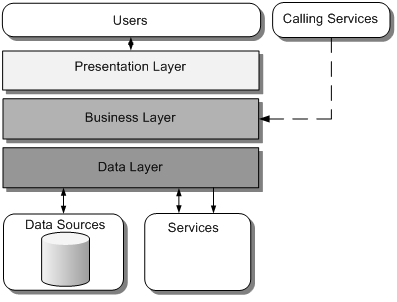
\includegraphics[scale=0.5]{img/layered-arch.PNG}
\caption{Arhitectură stratificată}
\label{fig:arhi_stratificata}
\end{figure}

Straturile aplicației pot fi aceeși mașină fizică (pe acelasi nivel) sau pot fi distribuite pe masini diferite (N-Nivele) și componentele din același nivel comunica cu componente din alte nivele prin interfețe bine definite. De exemplu o aplicație web tipică este alcătuită dintr-un nivel de prezentare (tot ceea ce ține de interfața grafică), un nivel de logică business și un nivel de acces de date. 

Principalele trăsături ale acestui stil includ:
\begin{itemize}
 \item Abstractizarea. Arhitectura stratificată abstractizează imaginea de ansamblu a sistemului ca și întreg în vreme ce oferă destule detalii pentru a înțelege rolurile și responsabilitățile fiecărui nivel individual și relația între ele.
 \item Encapsularea. Nici o presupune nu trebuie facută cu privire la tipurile de date, metode și proprietăți sau implementare în timpul proiectării, deoarece acestea nu vor fi expuse public.
 \item Nivele funcționale clar definite. Separarea funcționalității pe fiecare nivel este clară. Nivele superioare cum ar fi cel de prezentare trimit comenzi celor inferioare, cum ar fi cele de business și acces de date și poate reacționa la evenimente din aceste nivele, permițând fluxuri de date în ambele sensuri.
 \item Nivel ridicat de coeziune. Limitele bine definite ale responsabilității fiecărui nivel și asigurarea faptului ca fiecare nivel conține funcționalitatea strict legată de sarcinile acelui nivel contribuie  la maximizare nivelului de coeziune din acel nivel.
 \item Reutilizarea. Nivele inferioare nu depinde de cele superioare, permitând o posibilă reutilizare a acestora în cadrul altor scenarii.
 \item Cuplare slabă. Comunicarea între nivele este bazată pe abstractizare și evenimente pentru a oferi o cuplare slabă între acestea.
\end{itemize}

Exemple de aplicații stratificate includ aplicații de tip line-of-business (LOB) precum sisteme de contabilitate și administrarea clienților; aplicații web de tip enterprise și site-uri web și aplicații desktop sau agenți inteligenți cu un serer central pentru logica de business.

Tiparele de proiectare care susțin acest stil arhitectural sunt numeroase. De exemplu  tiparele "Separated Presentation" conțin a varietate large de tipare pentru manipularea interacțiunilor cu interfața grafică, logica de prezentare și business și datele aplicației cu care utilizatorul lucrează. Acesta permite designerilor sa lucreze la interfața grafica în vreme ce dezvoltatorii lucrează la codul care va orchestra totul. Împărțind funcționalitatea astfel crește sanșele de a test comportamentul individual al rolurilor. Principiile cheie ale acestui tipar sunt :

\begin{itemize}
	\item Separare responsabilității. Acest tipar împarte procesare interfeței grafice în roluri distincte; de exemplu MVC are 3 roluri diferite: modelul, view-ul și controller-ul. Modelul reprezintă datele; View-ul reprezintă interfața grafică; Controller manipulează cererile, modelul și efectuează alte operații.
	\item Notificării bazate pe evenimente. Tiparul observator este folosit pentru a trimite notificări View-ului când datele administrate de model se schimbă.
	\item Precesare delegată a evenimentelor. Controller-ul procesează evenimente lansate din interfața grafică.
\end{itemize}

Principalele beneficii ale acestui stil și tipar sunt :
\begin{itemize}
	\item Abstractizarea. Nivelele permit schimbări la nivel abstract. Se poate crește sau scădea nivelul de abstractizare al fiecărui nivel din stivă.
	\item Izolarea. Permite izolarea actualizărilor la nivele individuale pentru a reduce riscul și a minimiza impactul asupra sistemul ca și întreg.
	\item Administrarea. Separarea responsabilităților cheie ajută la identificarea depedențelor și organiează codul în blocuri mult mai gestionabile.
	\item Perfomanța. Distribuirea nivelelor pe mai multe mașini fizice poate crește scalabilitatea, fiabilitatea și performanța. 
	\item Reutilizarea. Rolurile promovează reutilizarea. De exemplu, în MVC, Controller-ul poate adesea fii refolosit de către alte View-uri pentru a crea un role specific sau un view personalizat bazat pe aceeași funcționalitate și date.
	\item Testarea. Posibilitatea sporită de testare rezultă din interfețe bine definite, cât și din posibilitatea de a trece de la o implementare la alta a interfeței nivelului.Tiparele de tip "Separated Presentation" permit construirea obiectelor de test pentru a simula comportamentul obiectelor concrete cum ar fi modelul, controller-ul sau view-ul în timpul testării.
\end{itemize}

Acest stil este adecvat cazului în care există nivele care poate fi reutilizate în alte aplicații, dacă există deja aplicații care expun procese de business prin interfețe de serviciu sau dacă aplicația este complexă și design-ul de nivel înalt impune o separare astfel încât echipele să se poată concentra pe arii diferite. Acest stil este potrivit și în cazul în care aplicația trebuie să fie diposnibilă pe tipuri diferite de clienți sau dispozitive sau dacă se dorește implementarea unor reguli și procese business complexe și configurabile.

Tiparul prezentat mai sus sporește posibilitatea de testare a aplicației și simplifică mentenanța funcționalității interfeței grafice și oferă posibilitatea separării sarcinilor de concepere a interfeței grafice de dezvoltarea logicii de business.

\section{Arhitectura bazată pe bus de mesaje}
Arhitectura bazată pe bus de mesaje descrie principiul folosirii unui sistem software care primește și trimite mesaje folosind unul sau mai multe canale de comunicare, astfel încât aplicațiile pot interacționa fără a fi nevoite să cunoască detalii. Este un stil de proiectare a aplicațiilor a caror interacțiune se realizează prin transmitere de mesaje (de obice asincron) prin intermediul unui bus comun. Implementările tipice ale acestui stil folosesc fie un ruter de mesaje fie tiparul "Publish/Subscribe" și sunt adesea implementate folosind sisteme de mesagerie de tip "cozi de mesaje". Multe implementări sunt alcătuite din aplicații individuale care comunică folosind o schemă comună și o infrastructură partajată pentru primirea și trimiterea de mesaje. Un bus de mesaje oferă posibilitatea de a gestiona :
\begin{itemize}
	\item Comunicații orientate pe mesaje.  Toate comunicațiile între aplicații se bazează pe mesaje care folosesc scheme cunoscute.
	\item Logică complexă de procesare. Operațiile complexe poate fi executate folosind un set de operațiuni mai mici, fiecare realizează o sarcină specifică, ca parte a unui proces cu mai multe etape.
	\item Modificări ale logicii de procesare. Deoarece interacțiunea cu bus-ul se bazează pe scheme și comenzi comune, se pot insera și scoate aplicații din bus pentru a schimba logica care este folosită pentru a procesa mesajele.
	\item Integrarea cu diverse medii. Folosind comunicarea orientată pe mesaje bazate pe standarde comune se pot crea interacțiuni între medii diferite cum ar fii Microsoft .Net și Java.
\end{itemize}

\begin{figure}[ht]
\centering
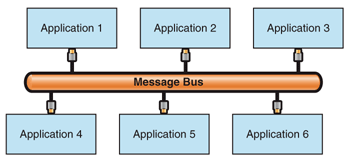
\includegraphics[scale=0.9]{img/message-bus.png}
\caption{Arhitectură bazată pe bus de mesaje}
\label{fig:arhi_bus_mesaje}
\end{figure}

Arhitecturile bazate pe bus de mesaje au fost folosite in cadrul procesărilor complexe. Acest design oferă o arhitectuă ce permite inserarea aplicațiilor în proces și îmbunătățeste scalabilitatea prin posibilitatea de a atașa numeroase instanțe alea aceleași aplicații în bus. Variații ale acestui stil sunt: 
\begin{itemize}
 \item Enterprise Service Bus (ESB). Bazată pe design cu bus de mesaje, ESB folosește servicii pentru comunicarea între bus și componentele atașate la bus. De obicei oferă servicii pentru convertirea mesaje între diferite formate, permițând clienților să folosească mesaje incompotabilie pentru a comunica între ei.
 \item Internet Service Bus (ISB). Similar cu precentul doar că în acest caz aplicațiile se află în cloud și nu pe rețeaua companiei. Un concept esențial al ISB reprezintă folosirea URI-urilor (Uniform Resource Identifiers) și a politicilor pentru controlarea rutării informației din cadrul proceselor aplicațiilor și serviciilor din cloud.
\end{itemize}

Principalele avantaje ale acestui stil sunt:
\begin{itemize}
 \item Extensibilitate. Aplicațiile pot fi adaugate sau înlăturate de pe bus fără a avea impact asupra aplicațiilor existente.
 \item Complexitate redusă. Complexitatea aplicațiilor este redusă, deoarece fiecare aplicație nu trebuie să cunoscă decât modul de interacțiune cu busul.
 \item Flexibilitate. Setul de aplicații care alcătuiesc un proces complex sau tiparele de comunicare între aplicații, pot fi ușor schimbate pentru a răspunde nevoilor de business, pur și simplu prin modificarea configurării sau a parametrilor care controlează rutarea.
 \item Cuplare slabă. Atât timp cât aplicațiile expun o interfață adecvată pentru comunicarea cu busul de mesaje, nu există nici o dependență față de aplicația în sine, aceasta permițând schimbări, actualizări și înlocuiri cu aplicații ce expun aceeași intefață.
 \item Scalabilitate. Mai multe instanțe ale aceeași aplicații pot fi atașate busului pentru a prelucra mai multe cereri în același timp.
 \item Simplitatea aplicației. Deși implementarea unui bus de mesaje adaugă complexitate infrastrucutrii, fiecare aplicație nu trebuie sa asigure decât o singură conexiune la bus în locul mai multora, către celălalte aplicații.
\end{itemize}

Acest stil arhitectural este potrivit cazurilor în care deja există aplicații care funcționează împreună pentru a realiza anumite funcții sau care combină mai multe sarcini într-o singură operație. Acest stil este adecvat dacă se dorește implementarea unei sarcini care necesită interacțiune cu aplicații externe sau aplicații găzduite pe medii diverse.

\section{Arhitectura orientată pe obiecte}
Arhitectura orientată pe obiecte este o pardigmă bazată pe divizarea responsabilităților dintr-o aplicație sau sistem pe obiecte individuale reutilizabile, fiecare conținând datele și comportamentul relevant obiectului. Un design orientat pe obiecte privește un sistem ca o serie de obiecte cooperând , în loc de un set de rutine sau instrucțiuni procedurale. Obiectele sunt discrete, independente și slab couplate; ele comunică prin interfețe, apelând metode sau accesând proprietăți ale obiectelor, sau trimițând si primind mesaje.
Principiile cheie ale stilui arhitectural obiect orientat sunt următoarele:

\begin{itemize}
 \item Abstractizare. Aceasta permite reducerea unei operațiuni complexe într-o generalizare ce reține caracteristicile de bază ale acesteia. De exemplu, o interfață abstractă poate fi o definiție bine cunoscută ce expune operațiuni legate de accesul la date folosind metode simple cum ar fi "get" sau "update". O altă formă de abstractizare ar putea fi metadatele folosite pentru a crea o mapare între două formate ce conțin date structurate.
 \item Compoziție. Obiectele pot asamblate pornind de la alte obiecte și pot ascunde obiectele interne din alte clase sau să le expună ca simple intefețe.
 \item Moștenire. Obiectele pot moșteni alte obiecte și folosi funcționalitatea din obiectul de bază sau sa o suprascrie pentru a implementa un nou comportament. În plus, moștenirea facilitează mentenanța și actualizările, deoarece schimbările în obiectul de bază propagă schimbările și în obiectele care îl moștenesc.
 \item Encapsularea. Obiectele expun funcționalitate numai prin metode, proprietăți și eveniment, dar ascund detalii interne cum ar fi starea sau variabile din alte obiecte. Aceasta ușureazp actualizarea și înlocuirea obiectelor, atât timp cât interfețele lor sunt compatibile, fără a afecta celălalte obiecte.
 \item Polimorfism. Aceasta permite suprascrierea comportamentului din tipul de bază care susține operații din cadrul aplicației implementând tipuri de noi care sunt interschimbabile cu obiectul existent.
 \item Decuplare. Obiectele pot fi decuplate de la consumator prin definirea unui interfețe abstracte pe care obiectele o pot implementa și pe care consumatorul o poate înțelege. Aceasta permite oferirea implementărilor alternative fără afectare consumatorilor interfeței.
\end{itemize}
Utilizări tipice ale acestui stil includ definirea unui obiect model care realizează operatii științifice comeplexe sau financiare, și a obiectelor care reprezintă artefacte din lumea reala dintr-un domeniu de business.

Beneficiile majore ale stilului orientat pe obiecte ar fi:
\begin{itemize}
 \item Inteligibilitatea. Mapează aplicația la obiecte mult mai apropiate de lumea reală, ceea ce o face mai inteligibilă.
 \item Reutilizarea. Oferă posibilitatea reutilizării codului prin intermediul polimorfismului și a abstractizării.
 \item Testarea. Posibilități sporite de testare prin intermediul encapsulării.
 \item Extensibilitatea. Folosirea encapsulării, a polimorfismului și a abstractizării izolează interfețele pe care obiectul le expun de schimbările asupra datelor.
 \item Nivel înalt de coeziune. Punând în obiect doar metode și funcționalități corelate și folosind diferite obiecte pentru diferite funcții se obține un nivel înalt de coeziune.
\end{itemize}

Acest stil se potrivește în cazul în care se dorește modelarea unui aplicații bazatî pe obiecte și acțiuni din lumea reală, sau dacă există deja obiectele și acțiunile care să se potrivească cu cerințele de design și operaționale.
El mai este adecvat și în cazul în cazre logica de business trebuie encapsulată alături de date în componente reutilizabile sau există logică de business complexă ce necesită abstractizare și comportament dinamic.

\section{Arhitectura orientată pe servicii}
Arhitectura orientată pe servicii crează posibilitatea expunerii funcționalității unei aplicații ca un set de servicii și crearea de aplicații care să folosească aceste servicii. Serviciile sunt slab cuplate deoarecere ele folosesc interfețe standard ce pot fi invocate, publicate și descoperite. Serviciile din cadrul SOA (Service Orientated Architecture) se concentrează pe oferirea unei interacțiuni bazate pe scheme și mesaje cu o aplicație prin interfețe care au scopul restrâns la aceasta și care nu sunt orientate pe componente sau obiecte. Un serviciu care respectă SOA nu ar trebuie sa fie considerat precum o componentă a unui furnizor de servicii. 

Stilul SOA poate să includă procese de business în servicii interoperabile folosind o gamă largă de protocoale și formate de date pentru comunicareaa informațiilor. Clienții și alte servicii pot accesa servicii local rulând la același nivel, sau pot accesa serviciile la distanță prin intermediul rețelei.

\begin{figure}[ht]
\centering
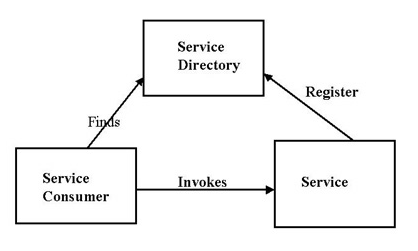
\includegraphics[scale=0.7]{img/soa.png}
\caption{Arhitectură orientată pe servicii}
\label{fig:arhi_orientata_servicii}
\end{figure}

Principiile cheie ale stilului SOA sunt:
\begin{itemize}
 \item Serviciile sunt autonome. Fiecare serviciu este menținut, dezvoltat, instalat și versionat în mod independent.
 \item Serviciile pot fi distribuite. Serviciile pot fi localizate oriunde pe rețea, local sau la distanță, atât timp cat rețeaua dispune de protocoalele necesare de comunicare.
 \item Serviciile sunt slab cuplate. Fiecare serviciu este independent față de celălalte și poate fi înlocuit și actualizat fără a întrerupe celălalte aplicații care îl folosesc atât timp cât interfețele sunt compatibile.
 \item Serviciile împarte schema și contractul, nu clasa. Serviciile partajează contracte și scheme atunci când comunică, și nu clase interne.
 \item Compatibilitatea se bazează pe politici. Politici în acest caz înseamnă definirea caracteristicilor precum transport, protocol și securitate.
\end{itemize}

Exemple tipice de aplicații orientate pe servicii includ cele legate de partajarea informației, manipularea proceselor multi-etapă precum sisteme de rezervare sau magazine online, ce expun date sau servicii specifice industriei prin intermediul unei rețele, creând colecții de informații din mai multe surse.

Beneficiile principale ale stilului SOA sunt:
\begin{itemize}
	\item Alinierea la domeniu. Reutilizarea serviciilor comune cu interfețe standard crește oportunitățile de business și tehnologice și reduce costurile.
	\item Abstractizarea. Serviciile sunt autonome și accesate printr-un contract formal, ce oferă cuplare slabă și abstactizare.
	\item Detectabilitatea. Serviciile pot expune descrieri care să permită altor aplicații și servicii să le localizeze și să construiască automat interfața.
	\item Interoperabilitatea. Deoarece protocoalele și formatele datelor sunt baze pe standarde din industrie, furnizorul și consumatorul servicilui pot fi construiți și instalați pe platforme diferite.
	\item Raționalizarea. Serviciile pot fi granulare pentru a oferi o funcționalitate specifică, mai degrabă decât să duplice funcționalitatea în cadrul mai multor aplicații.
\end{itemize}

Acest stil merită luat în considerare atunci când este diposnibil accesul la serviciile care se doresc a fi reutilizate; când serviciile pot fi cumpărate de la o companii terțe; când se dorește construirea aplicațiilor compuse dintr-o serie de servicii cu o singură interfață grafică; sau când se dorește crearea unei aplicații de tipul Software plus Services (S+S), Software as a Service (SaaS), sau bazate pe cloud. Stilul SOA este adecvat atunci trebuie asigurată comunicarea între segmentele unei aplicații și expuse funcționalități într-o manieră independentă de platformă, când se dorește utilizarea serviciilor centralizate precum autentificare sau expunerea serviciilor detectabile prin registre sau care pot fi utilizate de clienți care nu cunosc în prealabil interfețele.

\chapter{Microservicii}

Stilul arhitectural "micro servicii" reprezintă o abordare ce constă în dezvoltarea unuei aplicații ca o suită de mici servicii, fiecare rulând un proces independent și comunicând prin mecanisme simple, adesea resurse expuse prin API-uri via HTTP. Aceste servicii sunt construite în jurul nevoilor de business și instalate in mod automat. Există un minim necesar pentru o administrare centralizată a acestor servicii, care pot fii scrise folosind limbaje de programare și soluții de stocare diferite.

Pentru a explica mai bine microserviciile este utilă comparația cu stilul monolit: o aplicație construită ca o singură unitate. Aplicațiile de tip enterprise sunt adesea construite din trei părți: o interfață grafică către client (compusă din pagini HTML și javascript ce rulează in browser-ul utilizatorului), o bază de date (constituită din mai multe tabele dintr-un sistem de gestiune al bazei de date) și o parte de server. Aplicația server se ocupă de cererile HTTP, execută logica de business, extrage și actualizează datele din baza de date, selectează și populează paginile HTML care vor fi trimise browser-ului. Partea server este un \textit{monolit} - un singur executabil logic. Orice schimbare in sistem presupune construirea și instalrea unei noi versiune a aplicației.

O astfel de aplicație monolit este calea firească pentru construirea unui sistem. Toată logica pentru manipularea cererilor rulează în cadrul unui singur proces, permițând prin intermediul limbajului de programare împărțirea aplicației în clase, funcții și namespace-uri. Aceasta poate fi rulată și testată pe laptopul unui dezvoltator și instalată pe un mediu de producție folosind procese automatizate care să permită testarea acesteia. Aceasta poate fi scalată pe orizontală rulând mai multe instanțe în spatele unui load-balancer.

Aplicațiile monolit pot fi un real succes, însă un număr tot mai mare de oameni le constată limitările, odată cu creșterea numărului de servicii oferite în cloud. Ciclurile de schimbări sunt strâns legate - o schimbare făcută unei mici părți a aplicației, necesită recompilarea și instalarea intregului monolit.  În timp păstrarea unuei modularități bune devine dificilă, impiedicând astfel izolarea modificărilor. Scalarea implică scalarea întregii aplicații, nu a părtilor care necesită resurse în plus.

\begin{figure}[ht]
\centering
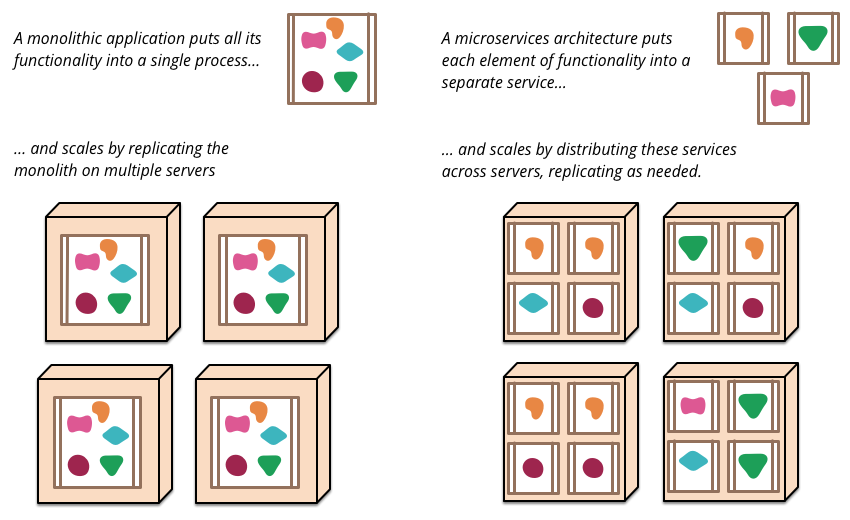
\includegraphics[scale=0.3]{img/sketch.png}
\caption{Arhitecturii monolit si microservicii}
\label{fig:arhi_mono_micro}
\end{figure}

Aceste considerente au dus la arhitectura microservicii: construirea aplicațiilor ca o suită de servicii. Pe lângă faptul ca serviciile pot fi instalate și scalate în mod independent, fiecare crează o limită fermă a modulului, permițând chiar și folosirea limbajelor de programare diferite, acestea putând fii gestionate de echipe diferite.

Acest stil arhitectural nu este o noutate, având rădăcini în principiile de proiectare ale Unix-ului, însă nu este îndeajuns de răspândit.

\section{Caracteristici ale arhitecturii microservicii}

Deși nu există o definiție formală a stilului arhitectural microservicii, însă se poate face o grupare a trăsăturilor comune arhitecturilor care se încadrează în acest tipar. Ca în cazul oricărei definiție care enumeră o serie de trăsături comune, aceste nu se vor regăsi în toate arhitecturile ce folosesc microservicii, dar este de așteptat ca majoritatea arhitecturilor să  prezinte o mare parte a acestora.

\subsection{Separarea prin intermediul serviciilor}

De-a lungul industriei software, a existat întotdeauna dorința de a construi sisteme prin conectarea diverselor componente, așa cum se întămplă în lumea reală. In ultimele decenii a existat un progres subsanțial în domeniul dezvoltării bibliotecilor reutilizabile. Când vorbim despre componente ne lovim de dificultatea de a defini ce este o componentă. Definiția pe care o putem da la acest moment este că o \textbf{componentă} este o parte software care poate fi înlocuită și actualizată în mod independent. 

Arhitecturile bazate pe microservicii folosesc librării, însă modalitatea principală prin care se face componentizarea este împărțirea pe servicii. Definim \textbf{bibliotecile} ca fiind componente ce funcționează împreună în cadrul unui program și deci au memorie comună, în vreme ce \textbf{serviciile} sunt componente ce rulează în cadrul unor procese diferite și care comunică prin mecanisme cum ar fi cereri de tip web sau \textbf{RPC} (Remote Procedure Call).

Unul din motivele pentru folosirea serviciilor ca și componente (mai degrabă decât biblioteci) este faptul că serviciile pot fi instalate în mod independent. În cazul unei aplicații constituită din mai multe biblioteci aparținând unui singur proces, o schimbare a oricărei component ar rezulta în reinstalarea întregii aplicații. Dacă însă aplicația este descompusă în mai multe servicii, este de așteptat ca modificările pe servicii să nu necesite decât reinstalări alei unui singur serviciu. Acest lucru nu este universal valabil, unele modificări ar putea impacta interfețe ale serviciilor necesitând o sincronizarea la nivelul mai multor servicii, însă ținta unei arhitecturi bazate pe microservicii este minimizarea acestui impact prin precizarea funcționalităților in cadrul contractelor.	

O altă consecință a folosirii serviciilor ca și componente este o intefațare mult mai explicită. Majoritatea limbajelor nu au un mecanism bun de definire a unei intefețe publice. Adesea, este doar documentația și disciplina utilizatorului care previn distrugerea încapsulării unei componente. Serviciile simplifică acest lucru folosind mecanisme explicite pentru apeluri la distanță.

Folosirea serviciilor în acest fel are și dezavantaje. Apelurile la distanță sunt mult mai costisitoare decât apleurile efectuate în cadrul aceluiași proces și de aceeas procedurile trebuie să fie mai puțin granulare, ceea ce implică și o dificultate de folosire. Schimbarea responsabilităților dintre componente este mai dificilă de făcut atunci când trebuie făcut trans-proces.

La o primă aproximare, se poate observa ca serviciile se mapează pe procese locale, dar această nu este decât o primă aproximare. Un serviciu poate fi constituit din mai multe procese care vor fi întotdeauna dezvoltate și instalate împreună, ca un proces de aplicație sau o o bază de date care va fi folosită doar de acel serviciu.

\subsection{Organizare în jurul nevoilor de business}

Când se dorește împărțirea unei aplicații în componente, adesea divizarea echipei se face în funcție de nivelul tehnologic, astfel formându-se echipe responsabile pentru interfața grafică, logica de server și baza de date. Când acestă împărțire este realizată, chiar și cele mai simple schimbări pot duce la proiecte realizate de mai multe echipe ceea ce consumă timp și bani. În 1967, Melvym Conawy afirma : "Orice organizație ce proiectează un sistem va produce un desgin care este o copie a structurii de comunicare a organizației".

\begin{figure}[ht]
\centering
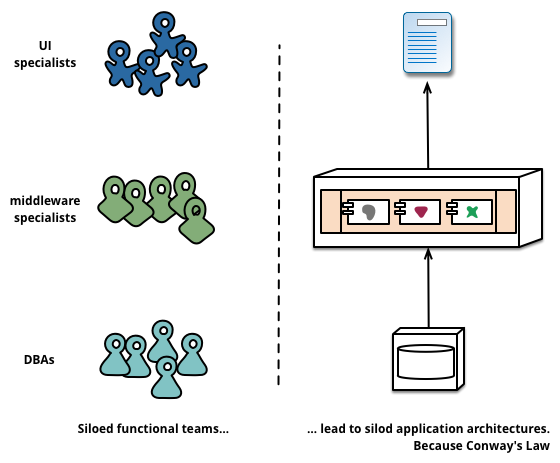
\includegraphics[scale=0.5]{img/conways-law.png}
\caption{Legea lui Conway}
\label{fig:legea_lui_conway}
\end{figure}

Abordarea separării componentelor diferă în cadrul microserviciilor, aceasta făcându-se ținând cont nevoile de business. Astfel de servicii preiau intreagă stivă tehnologică ce include interfața grafică, stocarea și orice colaborare externă. În consecință echipele sunt trans-funcționale, cuprinzând o plajă largă de cunoștințe necesare pentru dezvoltare: proiectarea interfeței grafice, baze de date și project management. 

\begin{figure}[ht]
\centering
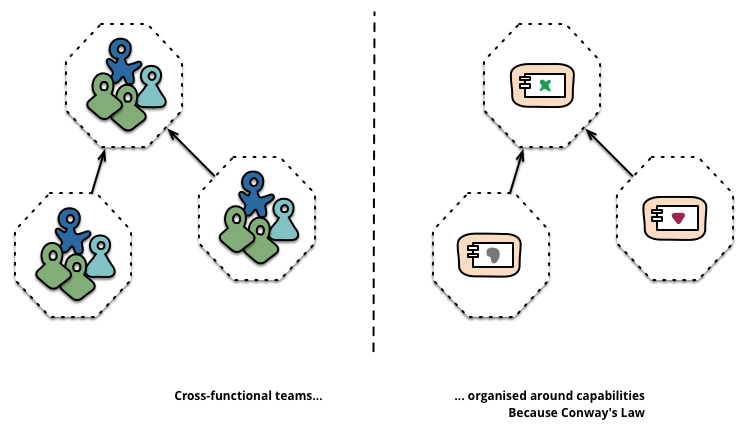
\includegraphics[scale=0.5]{img/cross-functional-team.png}
\caption{Echipe responsabile de servicii}
\label{fig:dist_respo_servicii}
\end{figure}

Aplicațiile mari monolit pot fi întotdeauna modularizate în jurul nevoilor de business, însă aceasta nu se întâmplă foarte des. Cu siguranță este de dorit ca o echipă mare ce construiește o aplicație monolit să fie împărțită în echipe mai mici concentrare pe liniile de business. Una din probleme care pot apărea aici este împărțirea liniilor de business în funcție de prea multe criterii. Dacă monolitul se extinde peste prea multe module poate deveni dificil ca membrii echipei să-și însușească aplicația. În plus se observă ca modularitatea implică un nivel mai mare de disciplină. Separarea mult mai explicită necesară componentelor bazate pe servicii sporește claritatea limitelor responsabilității echipei.

\subsection{Produse, nu proiecte}

Majoritatea efoturilor de dezvoltare pe care le vedem în cadrul unui proiect sunt concentrate pe livrarea unui program care tinde sa fie perceput ca fiind complet. Odata cu terminarea dezvoltării aplicația este predată unei echipe responsabile pentru mentenanță și echipa de proiect este desființată. 

Susținătorii microserviciilor tind să evite acest model, preferând în schimb noțiunea ca o echipă sa fie responsabil de produs pe întreaga sa viața. O sursă de inspirație pentru aceasta este sintagma din cadrul companiei Amazon: "you build it, you run it" unde echipa de dezvoltare își asumă responsabilitatea pentru mentenanța pe timpul producției. Aceasta îi aduce pe dezvoltatori în contact cu modul în care aplicația se comportă în producție și îmbunătățește contactul cu utilizatorii, preluând astfel o parte din efortul de mentenanță. 

Această mentalitate, se leagă și de dependința de nevoile de business. Mai degrabă decât să privim aplicațiile ca un set de funcționalități complete, există o relație permanentă unde întrebarea se pune cum poate soft-ul să ajute utilizatorii pentru a sporii capacitățile de business.

Nu există nici un motiv pentru care această abordare nu s-ar putea aplică și în cadru aplicațiilor monolit, dar granularitatea sporită oferită de servicii facilitează crearea relațiilor personale între dezvoltatori și utilizatori.

\subsection{Puncte termnale inteligente și bus-uri simple}

Pentru construirea unor structuri de comunicare între diferite procese există multe procese și abordări care se concentrează pe implementarea inteligenței în mecanismul de comunicare în sine. Un exemplu foarte bun este Entreprise Service Bus (\textbf{ESB}), aceste mecanisme oferind capacități complexe pentru rutarea mesajelor și aplicarea regulilor de business.

Microserviciile implică o altă abordare: puncte terminal inteligent și bus-uri simple (eng. "smart endpoints and dumb pipes"). Aplicațiile ce urmează aceste principii tind să fie cât mai decuplate, primind o cerere, aplicând logica adecvată și producând un răspuns. Acești pași sunt corelați folosind protocoale simple de tip REST mai degrabă decât cele complexe precum WS-Choreography, BPEL sau orchestrare prin intermediul unuei unelte centrale. 

Cele mai folosite două protocoale sunt HTTP cerere-răspuns folosind API-uri pentru accesarea resurselor și mecanisme simple de trimiterea mesajelor. Echipele care lucrează cu microservicii folosesc principiile și protocoalele pe baza caror a fost construit și web-ul. 

Al doilea mecanism folosit este cel al mesajelor transmise prin intermediul unui bus simplu. Infrastructura aleasă este adesea simplă (nu are decât rolul de a ruta mesajele) - implementări simple precum RabbitMQ sau ZeroMQ nu fac mai mult decât să pună la dispoziție un canal de comunicare asincron - inteligența rămânând în punctele terminale ce produc și consumă mesajele; în microservicii.

Într-un monolit, componentele execută instrucțiunile în cadrul aceluiași proces, iar comunicare între ele se face prin invocarea unei metode sau apelul unei funcții. Cea mai mare provocare în trecerea de la monolit la microservicii constă în schimbare șablonului de comunicare. O conversie de la apeluri în cadrul procesului la apeluri de tip RPC conduce la o comunicare excesivă care nu oferă o perfomanță bună. În schimb trebuie înlocuită comunicarea granulară cu o comunicare mai puțin selectivă.    

\subsection{Guvernare distribuit}

Una din consecințele unei guvernări centralizate este tendința de a standardiza tehnologia folosită. Experiența arată că aceasta abordare limitează flexibilitatea - "nu fiecare problemă este un cui și nu fiecare soluție este un ciocan". Se dorește folosirea uneltelor adecvate pentru a rezolva o problemă și în vreme aplicațiile monolit pot benefica într-o oarecare măsură de folosirea mai multor limbaje de programare, nu este ceva comun.  

Împărțirea componentelor unui monolith pe servicii implică alegerea limbajului de programare și a uneltelor adecvate pentru construirea fiecăruia. Bineînțeles, doar pentru că avem posibilitatea a construi sisteme eterogene din punct de vedere al tehnologiilor nu înseamnă că este ceva obligatoriu. 

Echipele care construiesc microservicii preferă o abordare diferită de cea standard. În loc să se folosească un set de standarde scrise, se preferă crearea de unelte pe care ceilalți dezvoltatori le pot folosi pentru a rezolva probleme similare cu cele cu care s-au confruntat. Acestea sunt distribuite in cadrul unor grupuri mai largi, dar nu în mod exclusiv folosindu-se modelul open-source. Popularitatea sporită a git și github a contribuit la răspândirea practicilor open source în cadrul companiilor. 

Netflix este un exemplu foarte bun de organizație care urmează această filozofie. Distribuind cod util și foarte bine testat sub forma unor librării încurajează alții dezvoltatori să rezolve probleme similare, însă lasă ușa deschisă pentru abordări diferite în caz de nevoie. Bibliotecile partajate tind să se concentreze pe probleme comune cum ar fi stocarea datelor, comunicarea inter-proces și după cum vom discuta în cele ce urmează automatizarea infrastructurii.

În cadrul comunității ce pratică microservicii, întârzierile sunt în mod particular neatractive. Aceasta nu implică o lipsă de importanță acordată contractelor de servicii, chiar dimpotrivă din moment ce ele tind să fie mai numeroase. Ele sunt doar privite dintr-o perspectivă diferită de administrare. Șabloane precum "Tolerant Reader" și "Consumer-Driver Contracts" sunt adesea aplicate microserviciilor. Aceastea facilitează o evoluție independentă a acestora. Folosirea contractelor orientate pe nevoile clienților ca și parte a proiectării crește nivelul de incredere și oferă un răspuns rapid asupra funcționării serviciului. Serviciul este apoi construit în vederea satisfacerii contractului. Aceste tehnici și apariția uneltelor adiacente, limitează nevoia centralizării contractelor prin scăderea cuplării temporale a serviciilor. 

\subsection{Managementul distribuit al datelor}

Management distribuit al datelor se poate face în mai multe feluri. La nivelul cel mai abstract, înseamnă că modelul conceptul va diferi de la un sistem la altul. Acesta este un scenariu tipic în cadrul aplicațiilor de tip enterprise, prespectiva departamentului de vânzări asupra datelor va fi diferită față de cea a echipei de suport. În acest caz informațiile despre un anumit client pot diferi. 

Aceasta este o problemă tipică care poate apărea la intregrarea diverselor aplicații, însă poate apărea și la nivelul aceleaiași aplicații. Un mod în care poate fi rezolvată această problemă este folosind șablonul "Bounded Design" din Domain-Driven Design (DDD). DDD împarte un domeniu complex în mai multe domenii limitate și mapează relațiile între acestea. Acest proces este util atât în cazul aplicațiilor monolit cât și în cel al microserviciilor, însă există o corelație naturală între serviciul și granițele contextului ce ajută la clarificarea și întărirea separării. 

Optarea pentru un model conceptual distribuit implică și un model distribuit pentru soluțiile de stocare. În vreme ce aplicațiile monolitice folosesc o singură bază de date pentru persistența datelor, în companiile mari se preferă o singură bază de date pentru o suită de aplicații - o parte a acestei decizii fiind legată de costul licenței. În cadrul microserviciilor se preferă folosirea propriei baze de date de către feicare serviciu în parte, fie instanțe diferite ale aceluiași sistem fie sisteme complet diferite - o abordare care se numește "Polyglot Persistence". Această abordare poate fi folosită și în cadrul aplicațiilor monolit, însă apare mai frecvent în cadrul microserviciilor. 

\begin{figure}[ht]
\centering
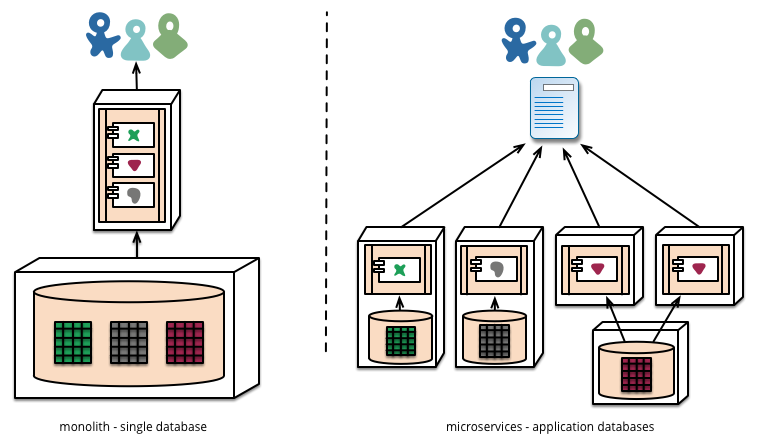
\includegraphics[scale=0.5]{img/decentralised-data.png}
\caption{Model distribuit al datelor}
\label{fig:model_dist_date}
\end{figure}

Folosirea unui model distribuit pentru pentru date implică și împărțirea responsabilității pentru mentenanța sistemelor. Abordarea comună pentru gestionarea actualizărilor a fost folosirea tranzacțiilor pentru asigurarea consistenței la nivelul mai multor resurse. Această abordare este folosită adesea în cadrul aplicațiilor de tip monolit. 

Astfel tranzacțiilor contribuie la asigurarea consistenței datelor, dar impune și o cuplare temporală, ceea ce este problematic în cazul folosirii mai multor servicii. Tranzacțiile distribuite sunt foarte greu de implementat și de aceea microserviciile se axează pe o coordonarea fără tranzacții între servicii, cu mențiunea că în acest caz consistența nu este garantată și că această problemă va fi adresată prin mecanisme de compensare. 

Faptul de a gestiona astfel inconsistențele este o nouă provocare pentru multe echipe de dezvoltare, dar este cea care adesea se pliează cel mai bine pentru cazurile de business. Adesea business-ul operează cu un anumit nivel de inconsistență pentru a răspunde repede la cereri, având la dispoziție mecanisme pentru trarea erorilor. Acest compromis rentează atât timp cât costul reparării greșelilor este mai mic decât costul pierderii anumitor informații de business. 	

\chapter{Automatizarea infrastructurii}

Tehnicile pentru automatizarea infrastructurii au evoluat foarte mult în ultimii ani - evoluția clodului și AWS - Amazon Web Services - în mod particular a redus foarte mult complexitatea operațională pentru gestionarea microserviciilor. 

Multe dintre produsele și sistemele folosind microservicii sunt construite de echipe cu experiență în Continous Delivery și predecesorul său, Continous Integration. Echipele ce construiesc astfel aplicațiile folosesc în mod extensiv tehnici de automatizare a infrastructurii. Acest lucru, denumit în literatura de specialitate \textbf{"pipeline"}, este ilustrat mai jos:

\begin{figure}[ht]
\centering
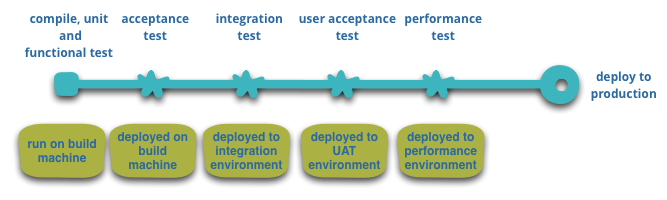
\includegraphics[scale=0.6]{img/basic-pipeline.png}
\caption{Pipeline}
\label{fig:arhi_componente}
\end{figure}

Câteva aspecte-cheie ale procesului de livrare continuă (e.g. Continous Delivery) sunt: încrederea cât mai mare în faptul calitatea software-ului dată de o suită foarte mare de teste automate; trecerea dintr-un mediu în altul în cadrul pipeline-ului înseamnă instalarea automată pe fiecare nou mediu. 

O aplicație monolit va fi compilată, testată și trecută prin aceste medii fără prea multe probleme. S-a constatat că investirea în automatizarea procesului de instalarea a unei aplicații în producție crește încrederea echipelor de a livra mult mai des pe acest mediu. Unul din obiectivele livrării continue este banalizarea procesului de instalare, astfel încât nu contează că se livrează una sau mai multe aplicații, lucrurile rămân la fel de simple. 




 


\end{document}